\documentclass[twoside,12pt]{mythesis} %this is the mythesis.cls file
% twoside,openright,versioninfo

% Consider:
% \newcommand{\ie}{i.\,e.}
% \newcommand{\Ie}{I.\,e.}
% \newcommand{\eg}{e.\,g.}
% \newcommand{\Eg}{E.\,g.}
\usepackage{graphicx}
\usepackage{amsmath}
\usepackage{booktabs}

%You might need to load other packages here...

%% Symbols
% unresolved:
\newcommand{\ud}{\mathrm{d}}
\newcommand{\drel}{\ensuremath{r_{\mathrm{rel}}}}
\newcommand{\nmax}{\ensuremath{n_\mathrm{max}}}

%Information for the title page
%Some of this is hard coded in mythesis.cls but you can over write if you need to
\title{My totally awesome thesis:\\%
  what I learned at university}
%
\author{My Name}
%
\month{\textsc{month}} \year{2014}
\previousdegrees{B.Sc., A University, 2000\\%
  M.Sc., Another University, 2003}
\degreetitle{Doctor of Philosophy}
\institution{Trinity College Dublin}
\school{School of Natural Sciences}
\department{Zoology/Botany}

%End of preamble.

\begin{document}

\maketitle %puts in your title

\chapter*{Abstract}
\chaptermark{abstract}
\addcontentsline{toc}{chapter}{Abstract}

This thesis template was kindly provided by \href{http://richfitz.github.io/}{Rich FitzJohn}
%

%%% Local Variables:
%%% TeX-master: "thesis"
%%% TeX-PDF-mode: t
%%% End:
 %inputs abstract.tex
\chapter*{Preface} %the * removes the numbers
\addcontentsline{toc}{chapter}{Preface}

Several chapters from my thesis have been published elsewhere:

\lettherebespace
\textsc{\Chapref{velociraptor}} has been previously published as:
%
\begin{previouspaper}
  FitzJohn R.G., Maddison W.P., and Otto S.P. 2009. Estimating
  trait-dependent speciation and extinction rates from incompletely
  resolved phylogenies.  Systematic Biology 58:595--611.
\end{previouspaper}
%
Here I explain what I did for this paper, and what the other coauthors did. Can just repeat this for each chapter if all are published already or in prep. Basically for anything you do with other people.

 %inputs preface.tex
\allcontents %tells it to make a table of contents with figure and table lists too
% There is currently a problem with spacing somewhere so that Table of
% Contents, List of Tables, and List of Figures have the wrong amount
% of space.  Others are OK though...
\chapter*{Acknowledgements}
\addcontentsline{toc}{chapter}{Acknowledgements}

I would like to acknowledge Dr Rich FitzJohn for letting me use his thesis template!

%%% Local Variables:
%%% TeX-master: "thesis.tex"
%%% TeX-PDF-mode: t
%%% End:
 %inputs acknowledgements.tex
\cleardoublepage
\mainbody

\chapter{Introduction}
\label{chap:introduction}%Note this label will be used to refer to the chapter throughout. So if you change the order of chapters it still knows this one is this file, but can call it chapter 1 or 2 or whatever depending on the order. S oti's better than calling it chapter 1.

\begin{quoteshrink}
  ``Really grandiose sounding quotes from Darwin always make a thesis feel more professional''
  \hfill{Natalie Cooper, p.~15}
\end{quoteshrink}

\noindent
Here is the introduction to the thesis.

\section{Subsection of my intro}

Here I introduce some concepts.

%The nice thing with LaTeX is you can leave notes in here, and/or stuff that you might include
%but might not. Rather than deleting it just comment out with %
%Should save time converting from thesis to papers and vice versa.

\section{Another subsection of my intro}

Here I introduce other concepts and provide a figure.

\begin{figure} %note figure will appear where LaTeX thinks it fits best. See http://en.wikibooks.org/wiki/LaTeX/Floats,_Figures_and_Captions if you need to tell it where to put the figure.
  \centering
  
\includegraphics[width = 30cm, height = 10cm, keepaspectratio=true]{ch1-introduction/Happy_smiley_face.png}
  \caption[Happy face because I finished]%this is what appears in table of contents
  {A nice happy face for you to enjoy.}%this is under the figure
\label{fig:happy}
\end{figure}

\section{Structure \& contents of this thesis}
In this thesis, I do some really cool stuff.
%
In \chapref{labstudy}, I do some lab work.
%
In \chapref{velociraptor}, I train a velociraptor to ride a hoverboard.
%
Finally, in \chapref{conclusions}, I close with a discussion of the
limitations of the methods used in the thesis, and suggest some future
directions.

 %This is a ch1-introduction.tex file with contents of intro chapter
\chapter[Lab study of my population]{Extensive lab study reveals exciting results in my study system}
\label{chap:labstudy}

\begin{abstract}
  Here is the chapter abstract.
\end{abstract}

\section{Introduction}

Here is the introduction.

\begin{figure}[p]
  \centering
  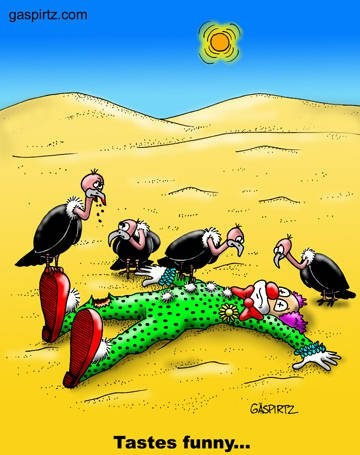
\includegraphics[width=.95\textwidth]{ch2-labstudy/Tastes_funny.jpg}%Note that this is the path for the folder
  %for chapter 2 that has the Tastes_funny.jpg file within it.
  \caption[Vultures]{Long explanation of the figure}
  \label{fig:vultures}
\end{figure}

\section{We all love a few equations}
We like to put in some equations for a bit of fun.
\begin{subequations}
  \label{eq:funequation1}
  \begin{align}
    \frac{\ud D_{Ni}}{\ud t} =& -(\lambda_i + \mu_i + q_{ij})D_{Ni}(t)
    + q_{ij}D_{Nj}(t) + 2\lambda_iE_i(t)D_{Ni}(t)
    \label{eq:funequation2}\\
    \frac{\ud E_i}{\ud t}
    =& \mu_i - (\lambda_i + \mu_i + q_{ij})E_i(t)
    + q_{ij}E_j(t) + \lambda_i E_i(t)^2
    \label{eq:funequation3}
  \end{align}
\end{subequations}
where $\lambda_i$ is the speciation rate in state $i$, $\mu_i$ is the
extinction rate in state $i$, and $q_{ij}$ is the rate of transition
from state $i$ to $j$ forward in time.

\section{Results}
We briefly present the results of our lab work and equations


\section{Discussion}

Here is the discussion
	%This is a ch2-labstudy.tex file with contents of intro chapter etc.
\chapter[Training velociraptors to hoverboard]{Extensive training of velociraptors confirms this was a terrible idea}
\label{chap:velociraptor}

\begin{abstract}
  Here is the chapter abstract.
\end{abstract}

\section{Introduction}

Here is the introduction.

\begin{figure}
  \centering
  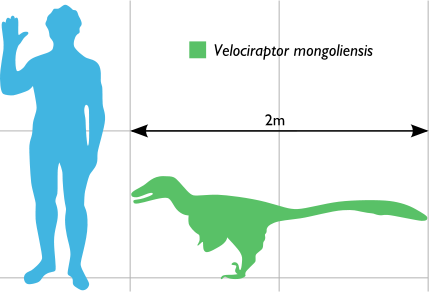
\includegraphics[width=.95\textwidth]{ch3-velociraptor/Velociraptor.png}%Note that this is the path for the folder for chapter 3
  \caption[Velociraptors to scale]{We use only small dinosaurs in these experiments to reduce disembowelment risks.}
  \label{fig:velociraptor}
\end{figure}

\section{Methods}

Let's just say we went through quite a lot of lab techs...

\section{Results}
We briefly present the results of our training; it didn't go so well...

\begin{table}
  \centering
  \caption[Results of dinosaur training]{
    The results showing how many times the three velociraptors were successfully trained, killed someone, or had to be excluded for other reasons.
  }
  \singlespacing
  \begin{tabular}{llrrr}
\toprule
Name & Success & Death & Excluded \\
\midrule
Dinosaur1  &   79 &   63 &  16 \\
Dinosaur2  &  286 &  250 &  36 \\
Dinosaur3  &   89 &   87 &   2 \\
\bottomrule
\end{tabular}
 %this is the .tex file with the table settings in ch3-velociraptor folder
  \label{tab:dinosaur}
\end{table}

\section{Discussion}

Here is the discussion. But we probably won't try this again with carnivorous dinosaurs.
	
\chapter{Conclusion}
\label{chap:conclusions}

So here are my conclusions...

\section{Future directions}
\label{sec:future-directions}

There's so much more to do!

\subsection{Improving my models}
\label{sec:bett-spec-models}

I'd like to write better analytical models! And try my methods on T rex too.
	

\formatbibliography %note there are only a few refs in this example in the appendix
\bibliographystyle{refstyle} %you may want to make a new reference style. This is refstyle.bst
\bibliography{refs-thesis} %you may also call you bibliography something different. This is refs-thesis.bib

\formatappendices
\chapter{Supplementary Information to \Chapref{labstudy}}%labstudy is the label for chapter 2.

\section{Additional cool equations}
%basically treat this the same as normal chapters
\label{sec:root-state-calc}
 
This probability is given by the likelihood given that the root is in state
$i$ divided by the sum of the likelihoods over both root states,
$D_{Ri}/(D_{R0}+D_{R1})$.  The overall likelihood is then:
\begin{equation}
  \label{eq:root}
  D_{R} = D_{R0}\frac{D_{R0}}{D_{R0} + D_{R1}} +
  D_{R1}\frac{D_{R1}}{D_{R0} + D_{R1}}
\end{equation}



\end{document}
